\documentclass{article}

\usepackage{fancyhdr}
\usepackage{extramarks}
\usepackage{amsmath}
\usepackage{amsthm}
\usepackage{amsfonts}
\usepackage{tikz}
\usepackage[plain]{algorithm}
\usepackage{algpseudocode}
\usepackage{enumitem}
\usepackage{multicol}
\usepackage{amsmath}
\usepackage[bottom]{footmisc}
\usepackage{multicol}
\usepackage{listings}
\usepackage{tabu}
% \usepackage[utf8]{inputenc}

% 
\usetikzlibrary{automata,positioning}

%
% Basic Document Settings
%




\topmargin=-0.45in
    \evensidemargin=0in
    \oddsidemargin=0in
    \textwidth=6in
    \textheight=9.0in
    \headsep=0.25in


\newenvironment{changemargin}[2]{%
        \setlength{\topsep}{0pt}%
        \setlength{\leftmargin}{5cm}%
        \setlength{\rightmargin}{5cm}%
        \setlength{\listparindent}{\parindent}%
        \setlength{\itemindent}{\parindent}%
        \setlength{\parsep}{\parskip}%

}


% \linespread{1.1}

\pagestyle{fancy}

%
% Homework Details
%   - Title
%   - Due date
%   - Class
%   - Section/Time
%   - Instructor
%   - Author
%

\newcommand{\hmwkTitle}{Project: Part C}
\newcommand{\hmwkDueDate}{November 16, 2018}
\newcommand{\hmwkClass}{Database Design and Implementation}
\newcommand{\hmwkClassTime}{}
\newcommand{\hmwkClassInstructor}{Professor Zhixiang Chen}
\newcommand{\hmwkAuthorName}{\textbf{David Caballero, Benjamin Garcia, Tomas Torres}}

%
% Title Page
%

\title{
    \vspace{2in}
    \textmd{\textbf{\hmwkClass:\ \hmwkTitle}}\\
    \normalsize\vspace{0.1in}\small{Due\ on\ \hmwkDueDate}\\
    \vspace{0.1in}\large{\hmwkClassInstructor}
    \vspace{3in}
}

\author{\hmwkAuthorName}
\date{}

\def\changemargin#1#2{\list{}{\rightmargin#2\leftmargin#1}\item[]}
\let\endchangemargin=\endlist 

% \renewcommand{\part}[1]{\textbf{\large Part \Alph{partCounter}}\stepcounter{partCounter}\\}

% %
% % Various Helper Commands
% %

% % Useful for algorithms
% \newcommand{\alg}[1]{\textsc{\bfseries \footnotesize #1}}

% % For derivatives
% \newcommand{\deriv}[1]{\frac{\mathrm{d}}{\mathrm{d}x} (#1)}

% % For partial derivatives
% \newcommand{\pderiv}[2]{\frac{\partial}{\partial #1} (#2)}

% % Integral dx
% \newcommand{\dx}{\mathrm{d}x}

% % Alias for the Solution section header
% \newcommand{\solution}{\textbf{\large Solution}}

% % Probability commands: Expectation, Variance, Covariance, Bias
% \newcommand{\E}{\mathrm{E}}
% \newcommand{\Var}{\mathrm{Var}}
% \newcommand{\Cov}{\mathrm{Cov}}
% \newcommand{\Bias}{\mathrm{Bias}}

\begin{document}

\maketitle

\pagebreak

\tableofcontents

\pagebreak

\begin{changemargin}{2cm}{2cm} 


\section{Introduction}

\subsection{Purpose}

This document we will descibe in detail the design of our TourneyDB web-based Data Management system. We will decompose the functionality of this design into interrelated modules that interact with each other through the transferring of data, we will break down these modules to the core tasks we want them to complete and show how they will be implemented as well as how they will interact with eachother.  

\subsection{Scope}

This is a preliminary design  for our TourneyDB prototype which will likely be modified if implementation presents any issue.

\subsection{Definitions, Acronyms, and Abbreviations}

\textbf{TourneyDB:} Our web-based software that will aid in the creation, management, and storage of the data relevant to running  a tournament.



\subsection{References}

TourneyDB will consist of three main modules: DataStorage, Data Processing, and UserInterface.



\end{changemargin}

\pagebreak


\section{System Overview}
Our system will provide almost all of the functionality required to handle the data necessary to run a tournament. It will handle user authentication and session management to protect the data created by individuals. It will allow for organizers to create tournaments, and allow guests to view tournaments in their areas, and view local players around them. It will automatically keep track of player performance and generate leaderboards that rank players among each other. It will also provide the functionality to track tournament status in real time.

\section{Decomposition Description}
    
Like most web applications our system will depend on 3 core modules, one that stores data, one that processes data, and one that presents that data to the user as well as intakes data from the user. These are represented in Figure \ref{fig:coremodules}.

\begin{figure}[H]
      \centering
      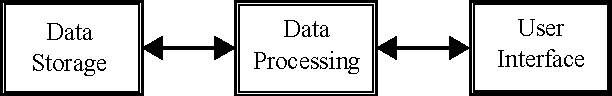
\includegraphics[width=.8\linewidth]{Figures/CoreModules.pdf}
      \caption{The three core modules of TourneyDB system. Arrows represent the transfer of data.}
      \label{fig:coremodules}
\end{figure}

\subsection{Data Storage Module}
This module stores all data needed by the TourneyDB system. It interacts directly with the data processing model by providing data needed to create views for the user, authenticate users, etc. It is a relational database consisting of tables that each represent an entity relevant to our system. Our Data Storage Module is represented by a diagram in Figure \ref{fig:datastoragemodule}.

\begin{figure}[H]
      \centering
      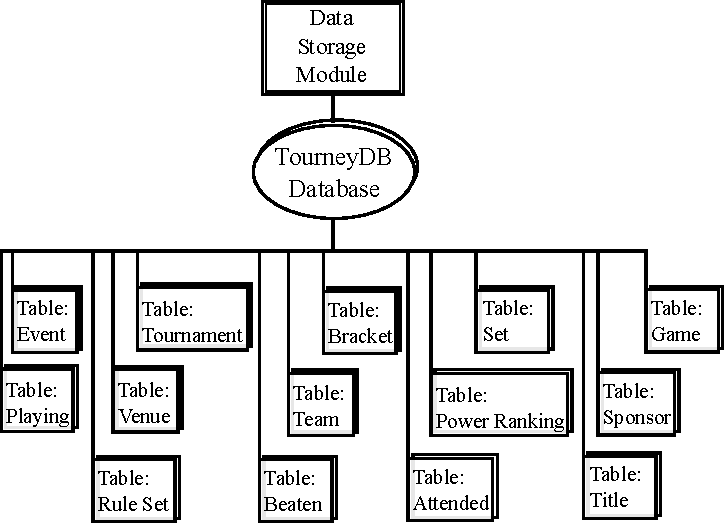
\includegraphics[width=.8\linewidth]{Figures/DataStorageModule.pdf}
      \caption{Breakdown of the Data Storage Module}
      \label{fig:datastoragemodule}
\end{figure}

\subsection{Data Processing Module}

This module will handle all server side processing of data. It will retrieve data from the Data Storage Module, and perform operations on it, such as sorting, formatting, etc. With the data provided from the User Interface it can retrieve specific data relevant to what the user wants. With the data retrieved from the Data Storage Module it can create dynamic web pages. This module will also handle the authentication of users. The Data processing module can further be broken down into specific function sets. These are \emph{User Authentication},  \emph{Database Connection Initiation}, \emph{Data Retrieval}, \emph{Data Update}, \emph{Data Filtering and Computation}, and \emph{Report Generation}.

\begin{enumerate}[noitemsep]
    \item \textbf{User Authentication and Authorization}: Allows the logging in of users of this site. Verfies the user has the permissions necessary for a certain action.
    \item \textbf{Database Connection Initiation}: Handles the initiation of the connection and authentication with the Data Storage Module
    \item \textbf{Data Retrieval}: Retrieves data from the Storage Module
    \item \textbf{Data Update}: Creates new data or modifies existing data in the Data Storage Module.
    \item \textbf{Data Filtering and Computation}: Performs operations on data such as computing certain statistics, sorting, filtering, etc.
    \item \textbf{Report Generation} Takes a request from the user interface module and generates a respective report.
\end{enumerate}



\begin{figure}[H]
      \centering
      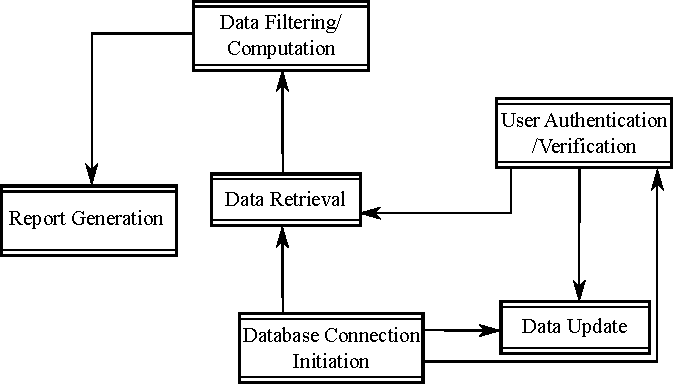
\includegraphics[width=.8\linewidth]{Figures/FunctionSet.pdf}
      \caption{Breakdown of the Data Storage Module}
      \label{fig:functionset}
\end{figure}



\subsection{User Interface Module}
The User Interface Module will be where a user directly interactis with our system. It will take data from the user that will be sent to the Data Processing Module, and it will present the data to the user in a viewable manner. There are 9 main pages that the user will interact with. Figure \ref{fig:uiflow} shows how these pages are linked to one another.

\begin{enumerate}[noitemsep]
    \item \textbf{Home Page}: First page a user sees when entering our site.
    \item \textbf{Login/Register}: Page where the player can enter their information to be authenticated or create a new account.
    \item \textbf{User Profile}: Page where the user can viee and update their own information.
    \item \textbf{My Tournaments}: Accessible through \emph{User Profile}. Shows the tournament created by a user.
    \item \textbf{Leaderboard}: Lets the user see the ranking of players that use the site.
    \item \textbf{Player View} Shows the information of another user.
     \item \textbf{Create Tournament}: The page for the creation of a tournament.
\end{enumerate}

\begin{figure}[H]
      \centering
      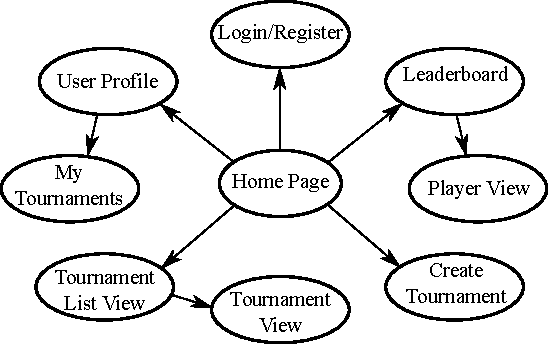
\includegraphics[width=.8\linewidth]{Figures/UIFlowchart.pdf}
      \caption{Flowchart of the User Interface}
      \label{fig:uiflow}
\end{figure}


\section{Dependency Description}
This section will describe both the hardware and th software that our TourneyDB system depends on.

\subsection{Data Storage Dependencies}
The Data Processing Module is a MySQL server hosted by AWS on a \emph{t2.micro} Ubuntu server instance. It is named tourneydb and has one authenticated user, authentication is necessary to start a connection with our database.




\begin{center}
  \begin{tabular}{ | l | c | r |}
    \hline
    \textbf{Hardware} & \textbf{Software}\\ \hline
    t2.micro instance  &  Ubuntu Server 18.04 \\
    1 vCPU  & MySQL 5.6.40 \\ 
    .5 GiB Memory  &  \\
    20 GB Storage  &  \\
    \hline
  \end{tabular}
\end{center}


\subsection{Data Processing Dependenies}
Our data processing module will be hosted on the same Ubuntu server. Our site will be hosted on a PHP 5.4.0 server running  on port 80. All data will be processed by PHP functions.

\begin{center}
  \begin{tabular}{ | l | c | r |}
    \hline
    \textbf{Hardware} & \textbf{Software}\\ \hline
    t2.micro instance  &  Ubuntu Server 18.04  \\
    1 vCPU  & PHP Server 5.4.0  \\
    .5 GiB Memory  &  \\
    20 GB Storage  &  \\
    \hline
  \end{tabular}
\end{center}

\subsection{User Interface Dependencies}
The User Interface Module is located on the same Ubuntu server, it will generate HTML documents dynamically using PHP and send those to clients requesting it. The structure and design will really on Bootstrop templates and CSS stylesheets.


\section{Interface Description}

\subsection{Data Storage Module Interface}
The MySQLi PHP libary will be used to connect and transfer data to the Data Storage Module. On loading our site, a connection will be created with our MySQL server through MySQLi, requiring authorized user credentials to be provided. We will execute queries and updates using SQL queries dynamically generated using PHP.

\subsection{Data Processing Module Interface}
Our PHP server will be accessible through port 80 of our Ubuntu server. It will be handed data through HTTP requests, and from there take the appropriate action such as loading of a new page, filtering of data, updating the Data Storage Module, \emph{etc.}

\subsection{User Interface Module Interface}
Our User Interface will be accessible through any desktop browser. It will use HTML forms to take in data from the user and send HTTP reqests to send these to our Data Processing Module.  


\section{Detailed Design}

\subsection{Application Program Design}
The root folder of our application will be in our TourneyDB directory. This folder will contain the PHP files that the server will run. Any resourcces needed such as images or videos will be in TourneyDB/resources.

\subsection{User Authentication Function Set}

\subsubsection{Authentication}
Authenticates a user with a username and a password

\end{document}